\clearpage
\section{Metodyka}

Największy nacisk w trakcie tworzenia pracy został położony na łatwość wdrożenia. 
W poniższych podrozdziałach przedstawiono kwestie, które należy wziąć pod uwagę
podczas projektowania rozwiązania, które ma tę cechę spełniać.

\subsection{Architektura systemu}

Wśród możliwych architektur systemów można wyłonić dwie najważniejsze gałęzie: 
architektura monolityczna lub oparta na mikrousługach, które są małymi, niezależnymi 
od siebie modułami, wspólnie ze sobą współpracującymi. Pierwsza z opcji opiera się 
na idei polegającej na tym, że wszystkie usługi oferowane przez dany system są zamknięte 
w jednym projekcie i funkcjonują jako całość. Druga możliwość opiera się na 
rozdzieleniu usług i umieszczeniu ich w oddzielnych modułach, które działają 
niezależnie od siebie. Obydwie architektury posiadają swoje wady i zalety i wybór 
jednej z nich zależy od specyficznych potrzeb każdego projektu. W tabeli 
\ref{tab:porownanie-architektur}. przedstawiono porównanie obydwu architektur 
\cite{newmanb2015}, które uwzględnia:

\begin{itemize} % lista nienumerowana
    \item Odporność systemu na awarie. Oferowane przez system usługi powinne być w każdym 
    momencie dostępne dla użytkowników
    \item Skalowalność. Potrzeba skalowania wynika ze zbyt dużego obciążenia dla jednego 
    lub większej liczby modułów w jednostce czasu. Brak dopasowania zasobów do 
    aktualnego zapotrzebowania może prowadzić do tego, że system nie będzie odpowiadał 
    na żądania użytkowników
    \item Łatwość wdrożenia. Architektura systemu nie powinna utrudniać wdrożenia nowych 
    funkcjonalności
    \item Zespół deweloperski. Architektura systemu nie powinna wymagać zatrudnienia 
    wielu programistów
\end{itemize}

    \begin{xltabular}{1\textwidth} { 
        | >{\arraybackslash}c 
        | >{\arraybackslash}X 
        | >{\arraybackslash}X | }
        \caption{Porównanie popularnych architektur systemów} \label{tab:porownanie-architektur} \\
        \hline
       Cecha & System monolityczny & System oparty na architekturze mikrousługowej \\
        \hline
       Odporność systemu na awarie & 
       W przypadku awarii w jednym punkcie, cały system przestaje działać & 
       Awaria jednego z modułów niekoniecznie musi oznaczać niesprawność całego systemu \\
       \hline
       Skalowalność & 
       Wymusza zwiększanie liczby uruchomionych instancji systemu, nawet w przypadku silnego 
       zapotrzebowania jedynie na część oferowanych usług & 
       Możliwość zwiększania liczby instancji tylko tych mikrousług, które w danym momencie są 
       silnie obciążone \\
      \hline
      Łatwość wdrożenia &
      Nawet mała zmiana w kodzie systemu monolitycznego wymaga ponownego wdrożenia całego 
      kodu &
      Możliwość szybkiego wdrożenia poprawek w obrębie danego mikroserwisu \\
      \hline
      Zespół deweloperski &
      Rozbudowany projekt zazwyczaj wymaga zespołu liczącego setki programistów, co 
      utrudnia komunikację i zmniejsza efektywność pracy &
      Nie wymaga rozbudowanego zespołu, możliwość oddelegowania małej grupy pracowników 
      do oddzielnych mikroserwisów \\
      \hline
    \end{xltabular}

Biorąc pod uwagę założenia dotyczące projektu, lepszą decyzją jest wykorzystanie architektury
mikrousługowej. Zestawienie z tabeli \ref{tab:porownanie-architektur} jasno wskazuje, że 
konsekwencją dokonanego wyboru jest szybsze wdrożenie kolejnych wersji systemu.

\subsubsection{Serwisy zorientowane usługowo}

Docelowo, system oparty na architekturze mikrousługowej powinien składać się z mikroserwisów 
zorientowanych usługowo (ang. \textit{service-oriented architecture}). Stanowią one 
konstrukcję, w której wiele modułów współpracuje ze sobą w celu zapewnienia zbioru 
funkcjonalności. Serwis oznacza tutaj oddzielny proces pracujący na danej maszynie. 
Procesy te komunikują się ze sobą przez sieć.

\subsubsection{Sprzężenie serwisów}

Architektura mikrousługowa opiera się na tym, że poszczególne mikroserwisy działają 
niezależnie od siebie. Dzięki temu zmiany wprowadzone w jednym z modułów nie powinny 
wymagać zmian w drugim. Ponadto wdrożenie danego mikroserwisu nie powinno wymagać 
jednoczesnego wdrożenia innych. O tak rozdzielonych mikroserwisach mówi się, że są ze sobą 
luźno sprzężone (ang. \textit{loose coupling}). Prawidłowo skonstruowany mikroserwis powinien 
wiedzieć jedynie tyle, w jaki sposób może komunikować się z innymi mikroserwisami w celu 
uzyskania wymaganych danych.

\subsubsection{Spójność mikroserwisów}
W prawidłowo skonstruowanym systemie mikrousługowym funkcjonalność związana ze 
sobą (np. w kontekście biznesowym) jest umieszczona w jednym miejscu. O tak 
zaprojektowanych modułach mówi się, że są one spójne (ang. \textit{high cohesion}). 
Przykładem 
błędnej implementacji może być edycja danych osobowych klienta w wielu mikroserwisach. 
Wtedy zmiana w jednym module może wymagać zmiany w innych.

\subsubsection{Wyznaczanie granic między mikroserwisami}

Jednym z wyzwań stojących przed projektantem systemu jest wyznaczenie granic między
mikroserwisami. Każdy z mikroserwisów powinien być niezależny od innych. Aby to osiągnąć, należy
skupić się na wyznaczeniu odrębnych modeli danych wykorzystywanych przez system
\cite{delatorre2015}.
Każdy z modeli może odgrywać różną rolę w kontekście biznesowym. Dzięki podziałowi
modelu danych na mniejsze fragmenty można utworzyć oddzielne moduły, każdy z których
będzie odpowiedzialny za osobny fragment. W konsekwencji uzyskiwana jest niezależność
mikroserwisów. Mogą one komunikować się między sobą w celu otrzymania wymaganych informacji.

\subsubsection{Architektura systemu do zarządzania energią w pomieszczeniach biurowych}

Opierając się na poprzednich podrozdziałach oraz w oparciu o założenia utworzono 
architekturę systemu będącego rezultatem tej pracy inżynierskiej. Rysunek 
\ref{fig:architektura-systemu} przedstawia pełny zestaw modułów składających się na 
całość rozwiązania:

\begin{figure}[h]
    \centering
    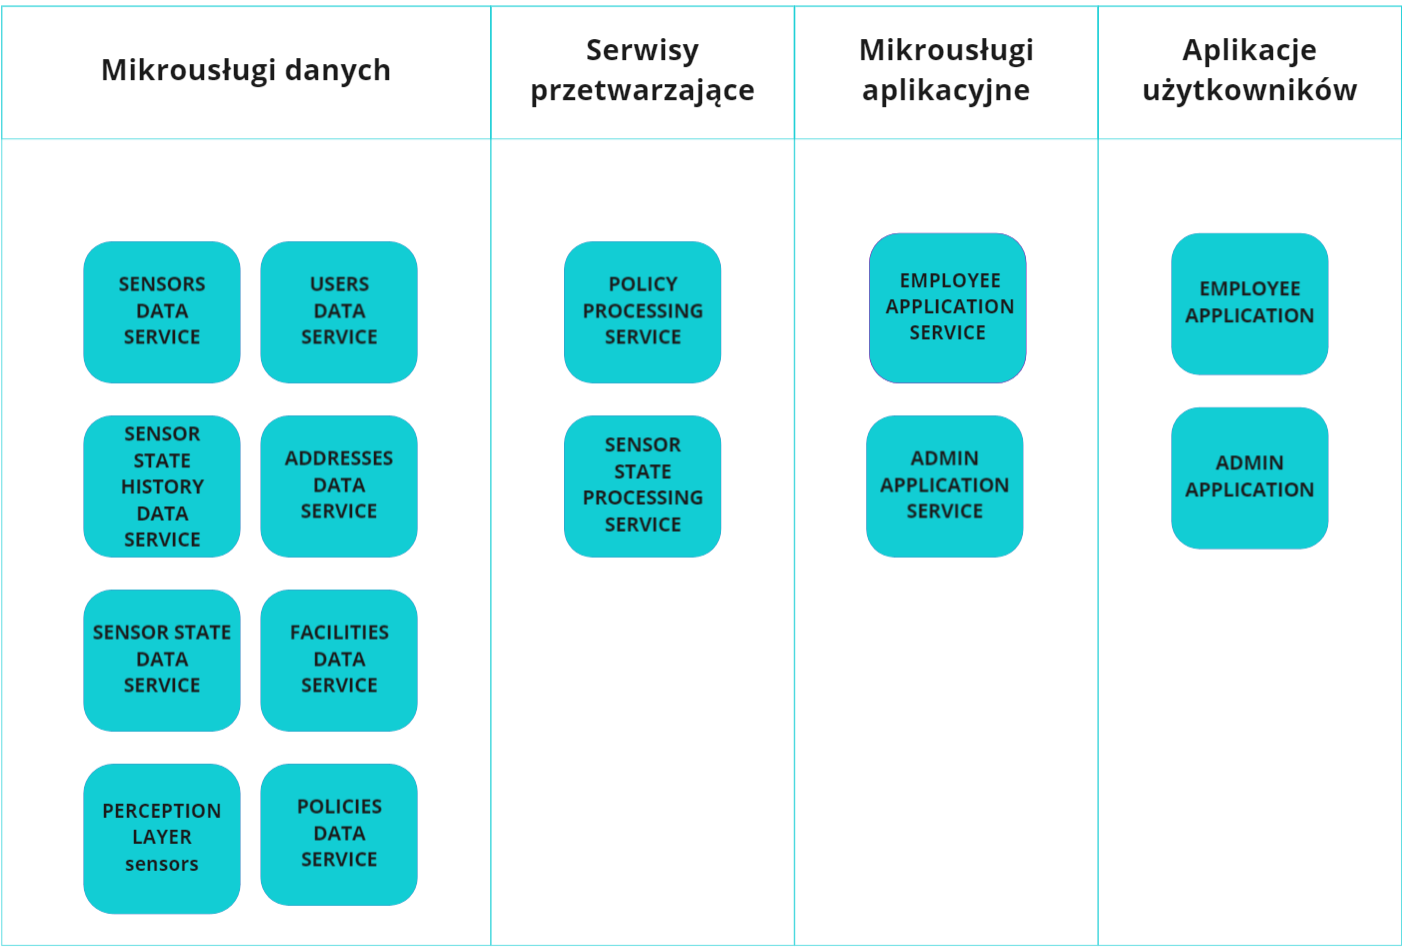
\includegraphics[width=1\textwidth]{architektura.jpg}
    \caption{Architektura systemu. Opracowanie własne}
    \label{fig:architektura-systemu}
\end{figure}

W tabeli \ref{tab:mikroserwisy-danych} opisano rolę mikroserwisów danych.

    \begin{xltabular}{1\textwidth} { 
        | >{\raggedright\arraybackslash}c        
        | >{\raggedright\arraybackslash}X | }
        \caption{Mikroserwisy danych} \label{tab:mikroserwisy-danych} \\
        \hline
       Nazwa & Funkcja \\
       \hline
       Addresses data service & 
       Przechowuje adresy organizacji oraz poszczególnych budynków \\
       \hline
       Facilities data service &
       Przechowuje szczegółowe dane dotyczące budynków \\
       \hline
       Policies data service & 
       Przechowuje reguły określające oczekiwaną wartość mierzonych parametrów \\
       \hline
       Sensors data service &
       Przechowuje szczegółowe dane dotyczące wykorzystywanych czujników \\
       \hline
       Sensor state history data service &
       Przechowuje historyczne pomiary z poszczególnych czujników \\
       \hline
       Sensor state data service &
       Przesyła pomiary od czujników \\
       \hline
    \end{xltabular}

Poza mikroserwisami danych aplikacja posiada również mikroserwisy przetwarzające 
dane, opisane w tabeli \ref{tab:serwisy-przetwarzajace}:

    \begin{xltabular}{1\textwidth} { 
        | >{\raggedright\arraybackslash}c        
        | >{\raggedright\arraybackslash}X | }
        \caption{Mikroserwisy przetwarzające} \label{tab:serwisy-przetwarzajace} \\
        \hline
       Nazwa & Funkcja \\
       \hline
       Sensor state processing service & 
       Otrzymuje dane z czujników. Zajmuje się ich prawidłowym zapisaniem, po czym wysyła 
       je dalej do PPS \\
       \hline
       Policy processing service &
       Przetwarza dane z czujników. Porównuje pomiary rzeczywiste z oczekiwanymi, które 
       zostały określone w regułach \\
       \hline
    \end{xltabular}

Na system składają się także mikroserwisy aplikacyjne opisane w tabeli \ref{tab:mikroserwisy-aplikacyjne}:

    \begin{xltabular}{1\textwidth} { 
        | >{\raggedright\arraybackslash}c        
        | >{\raggedright\arraybackslash}X | }
        \caption{Mikroserwisy aplikacyjne} \label{tab:mikroserwisy-aplikacyjne} \\
        \hline
       Nazwa & Funkcja \\
       \hline
       Employee application service & 
       Mikrousługa aplikacyjna dla aplikacji pracowników. Oferuje usługi umożliwiające 
       zarządzanie kontem, tworzenie własnych reguł dla pomieszczeń przypisanych do 
       konkretnego użytkownika oraz sprawdzanie ich aktualnego stanu \\
       \hline
       Admin application service &
       Mikrousługa aplikacyjna dla aplikacji administratorów. Oferuje wszystkie usługi 
       udostępniane pracownikom, a ponadto usługi umożliwiające zarządzanie informacjami 
       dotyczącymi organizacji, budynków, pomieszczeń i czujników \\
       \hline
    \end{xltabular}

Ostatnimi elementami systemu są aplikacje dla poszczególnych ról użytkowników, opisane 
w tabeli \ref{tab:aplikacje-uzytkownikow}:

    \begin{xltabular}{1\textwidth} { 
        | >{\raggedright\arraybackslash}c        
        | >{\raggedright\arraybackslash}X | }
        \caption{Aplikacje użytkowników} \label{tab:aplikacje-uzytkownikow} \\
        \hline
       Nazwa & Funkcja \\
       \hline
       Employee application & 
       Oferuje graficzny interfejs do interakcji z mikrousługą aplikacyjną pracowników \\
       \hline
       Admin application &
       Oferuje graficzny interfejs do interakcji z mikrousługą aplikacyjną administratorów \\
       \hline
    \end{xltabular}

\subsection{Zwinne zarządzanie}

Podczas tworzenia systemu zastosowano metodykę Scrum, będącą metodyką zarządzania projektem
typu zwinnego\cite{sommerville2011}. Cechuje się iteracyjnym podejściem do implementacji systemu.
Metodyka zakłada trzy fazy rozwoju. W pierwszej definiuje się ogólne założenia 
dotyczące projektu, zakłada jego cele oraz zastosowania. Przygotowuje się także
architekturę systemu, składającą się z mikroserwisów, baz danych, brokerów wiadomości.
W następnej fazie następuje seria cykli tzw. sprintów, gdzie każdy cykl oznacza
iteracyjne wzbogacanie systemu o nowe funkcjonalności. W ostatniej fazie następuje
zakończenie rozwoju projektu, jego udokumentowanie, po czym spisuje się nabyte
doświadczenia.

Na początku każdego ze sprintów definiowany jest zakres pracy, który powinien zostać
ukończony. Na podstawie ustalonych wymagań dzieli się pracę na mniejsze, niezależne
od siebie fragmenty. Następnie każdy członek zespołu deweloperskiego wybiera jedno
z dostępnych zadań i implementuje rozwiązanie. Sprint zazwyczaj trwa od dwóch do
czterech tygodni.